% THIS IS SIGPROC-SP.TEX - VERSION 3.1
% WORKS WITH V3.2SP OF ACM_PROC_ARTICLE-SP.CLS
% APRIL 2009
%
% It is an example file showing how to use the 'acm_proc_article-sp.cls' V3.2SP
% LaTeX2e document class file for Conference Proceedings submissions.
% ----------------------------------------------------------------------------------------------------------------
% This .tex file (and associated .cls V3.2SP) *DOES NOT* produce:
%       1) The Permission Statement
%       2) The Conference (location) Info information
%       3) The Copyright Line with ACM data
%       4) Page numbering
% ---------------------------------------------------------------------------------------------------------------
% It is an example which *does* use the .bib file (from which the .bbl file
% is produced).
% REMEMBER HOWEVER: After having produced the .bbl file,
% and prior to final submission,
% you need to 'insert'  your .bbl file into your source .tex file so as to provide
% ONE 'self-contained' source file.
%
% Questions regarding SIGS should be sent to
% Adrienne Griscti ---> griscti@acm.org
%
% Questions/suggestions regarding the guidelines, .tex and .cls files, etc. to
% Gerald Murray ---> murray@hq.acm.org
%
% For tracking purposes - this is V3.1SP - APRIL 2009

\documentclass{edm_template}
\usepackage[T1]{fontenc}
\usepackage[utf8]{inputenc}
\usepackage{algorithm,caption,algpseudocode}
\usepackage{hyperref}
\usepackage{color}
\usepackage{array}

\newcommand\alert[1]{\textcolor{red}{#1}}

\begin{document}

\title{Predicting Performance on Dichotomous Questions:\\Comparing Models for Large-Scale Adaptive Testing}
%\subtitle{[Extended Abstract]
%\titlenote{A full version of this paper is available as
%\textit{Author's Guide to Preparing ACM SIG Proceedings Using
%\LaTeX$2_\epsilon$\ and BibTeX} at
%\texttt{www.acm.org/eaddress.htm}}}
%
% You need the command \numberofauthors to handle the 'placement
% and alignment' of the authors beneath the title.
%
% For aesthetic reasons, we recommend 'three authors at a time'
% i.e. three 'name/affiliation blocks' be placed beneath the title.
%
% NOTE: You are NOT restricted in how many 'rows' of
% "name/affiliations" may appear. We just ask that you restrict
% the number of 'columns' to three.
%
% Because of the available 'opening page real-estate'
% we ask you to refrain from putting more than six authors
% (two rows with three columns) beneath the article title.
% More than six makes the first-page appear very cluttered indeed.
%
% Use the \alignauthor commands to handle the names
% and affiliations for an 'aesthetic maximum' of six authors.
% Add names, affiliations, addresses for
% the seventh etc. author(s) as the argument for the
% \additionalauthors command.
% These 'additional authors' will be output/set for you
% without further effort on your part as the last section in
% the body of your article BEFORE References or any Appendices.

\numberofauthors{5} %  in this sample file, there are a *total*
% of EIGHT authors. SIX appear on the 'first-page' (for formatting
% reasons) and the remaining two appear in the \additionalauthors section.
%
\author{
% You can go ahead and credit any number of authors here,
% e.g. one 'row of three' or two rows (consisting of one row of three
% and a second row of one, two or three).
%
% The command \alignauthor (no curly braces needed) should
% precede each author name, affiliation/snail-mail address and
% e-mail address. Additionally, tag each line of
% affiliation/address with \affaddr, and tag the
% e-mail address with \email.
%
% 1st. author
\alignauthor{\parbox{5.5cm}{\centering Jill-Jênn Vie, Fabrice Popineau, Yolaine Bourda}}\\
       \affaddr{LRI -- Bât. 650 Ada Lovelace}\\
       \affaddr{Université Paris-Sud}\\
       \affaddr{91405 Orsay, France}\\
       \email{\parbox{5.5cm}{\{jjv, popineau, bourda\}@lri.fr}}
% 2nd. author
%\alignauthor
%\phantom{Fabrice Popineau}%\\
%       \affaddr{\phantom{LRI -- Bât. 650 Ada Lovelace}}%\\
%       \affaddr{\phantom{Université Paris-Sud}}%\\
%       \affaddr{\phantom{91405 Orsay, France}}%\\
%       \email{\phantom{fabrice.popineau@centralesupelec.fr}}
% 3rd. author
\alignauthor Jean-Bastien Grill\\
       \affaddr{Inria Lille - Nord Europe}\\
       \affaddr{40 avenue Halley}\\
       \affaddr{59650 Villeneuve-d'Ascq, France}\\
       \email{grill@clipper.ens.fr}
% 4th. author
\alignauthor Éric Bruillard\\
       \affaddr{ENS Cachan -- Bât. Cournot}\\
       \affaddr{61 av. du Président Wilson}\\
       \affaddr{94235 Cachan, France}\\
       \email{eric.bruillard@ens-cachan.fr}
}
% 5th. author
%\alignauthor
%\phantom{Yolaine Bourda}%\\
%       \affaddr{\phantom{LRI -- Bât. 650 Ada Lovelace}}%\\
%       \affaddr{\phantom{Université Paris-Sud}}%\\
%       \affaddr{\phantom{91405 Orsay, France}}%\\
%       \email{\phantom{yolaine.bourda@centralesupelec.fr}}
%}
% There's nothing stopping you putting the seventh, eighth, etc.
% author on the opening page (as the 'third row') but we ask,
% for aesthetic reasons that you place these 'additional authors'
% in the \additional authors block, viz.
% \additionalauthors{Additional authors: John Smith (The Th{\o}rv{\"a}ld Group,
% email: {\texttt{jsmith@affiliation.org}}) and Julius P.~Kumquat
% (The Kumquat Consortium, email: {\texttt{jpkumquat@consortium.net}}).}
\date{February 9, 2015}
% Just remember to make sure that the TOTAL number of authors
% is the number that will appear on the first page PLUS the
% number that will appear in the \additionalauthors section.

\maketitle
\begin{abstract}
Computerized adaptive testing (CAT) is a mode of testing which has gained increasing popularity over the past years. It selects the next question to ask to the examinee in order to evaluate her level efficiently, by using her answers to the previous questions.
Traditionally, CAT systems have been relying on item response theory (IRT) in order to provide an effective measure of latent abilities in possibly large-scale assessments.
More recently, from the perspective of providing useful feedback to examinees, other models have been studied for cognitive diagnosis. One of them is the q-matrix model, which draws a link between questions and examinee knowledge components.
In this paper, we define a protocol based on performance prediction to evaluate adaptive testing algorithms. We use it to evaluate q-matrices in the context of assessments and compare their behavior to item response theory.
Results computed on three real datasets of growing size and of various nature suggest that tests of different type need different models.
% Results computed on three real datasets of growing size and of different nature suggest that according to the type of test, either the Rasch model or the q-matrix performs the best.
\end{abstract}

%% A category with the (minimum) three required fields
%\category{H.4}{Information Systems Applications}{Miscellaneous}
%\category{}{Student assessment}{Adaptive testing}
%%A category including the fourth, optional field follows...
%\category{D.2.8}{Software Engineering}{Metrics}[complexity measures, performance measures]
%
%\terms{Theory}

\keywords{Adaptive assessment, computerized adaptive testing, cognitive diagnosis, item response theory, q-matrices} % NOT required for Proceedings

\section{Introduction}
Automated assessment of student answers has lately gained popularity in the context of online initiatives such as massive online open courses (MOOCs). Such systems must be able to rank thousands of students for evaluation or recruiting purposes and to provide personal feedback automatically for formative purposes.

For computerized adaptive tests (CAT), item response theory (IRT) provides the most common models~\cite{Desmarais2012}. IRT provides a framework to evaluate the performance of individual questions, called \emph{items}, on assessments~\cite{Hambleton1991}. When the intention is more formative, examinees can receive a detailed feedback, specifying which knowledge components (KCs) are mastered and which ones are not~\cite{Cheng2009}. Most of these models rely on a q-matrix specifying for each question the different KCs required to solve it.

We propose a protocol to evaluate adaptive testing algorithms and use it to compare the performances of the simplest IRT model, the 1-parameter logistic one, commonly known as Rasch model, with the simplest Q-matrix model. We expect to answer the following question: given a budget of questions of a certain dataset asked according to a certain adaptive selection rule, which model performs the best at predicting the answers of the examinee over the remaining questions? We managed to get satisfactory results, enabling us to state that no model dominates in all cases: according to the type of test, either the Rasch model or the q-matrix performs the best.

% the simple item criterion of maximizing Fisher information and a greedy one-step approach.

\section{Background and Related Work}

\subsection{Item Response Theory: Rasch Model}

The Rasch model estimates the latent ability of a student by a unique real number $\theta$ modeled by a random variable and characterizes each question by one real number: its difficulty $d$, corresponding to the ability needed to answer the question correctly. Knowing those parameters, the probability of the event ``the student of ability $\theta$ answers the question of difficulty $d$ correctly'', denoted by \emph{success}, is modeled by:
\[ \Pr\{success|\theta\} = \frac1{1+e^{-(\theta - d)}}. \]
The aim is first to optimize the parameters $d_j$ for each question $j$ and $\theta_i$ for each student $i$ in order to fit a given train dataset. Then, throughout the test, a probability distribution over $\theta_i$ is updated after each question answered, using the Bayes' rule.

\subsection{Cognitive Diagnosis Model: Q-matrix}

We now present a model that tries to be more informative about the student's knowledge components. Every student is modeled by a vector of binary values $(a_1, \ldots, a_K)$, called \emph{knowledge vector}, representing her mastery of $K$ distinct KCs. A q-matrix $Q$ \cite{Tatsuoka1983} represents the different KCs involved in answering every question. In the NIDA model considered here~\cite{Desmarais2012}, $Q_{ij}$ is equal to 1 if the KC $j$ is required to succeed at question $i$, 0 otherwise. More precisely, we denote by $s_i$ ($g_i$) the \emph{slip} (\emph{guess}) parameter of item $i$. The probability of a correct response at item $i$ is $1 - s_i$ if all KCs involved are mastered, $g_i$ if any required KC is not mastered.

% Determining the best q-matrix that fits a given dataset is currently an open field of research, the state of the art being hill-climbing techniques~\cite{Barnes2005}, non-negative matrix factorization~\cite{Desmarais2011} or the EM algorithm~\cite{Huebner2010}. 

The KCs are considered independent, thus the student's knowledge vector is implemented as a vector of size $K$ indicating for each KC the probability of the student to master it. Throughout the test, this vector is updated using Bayes' rule. From this probability distribution and with the help of our q-matrix, we can derive the probability for a given student to answer correctly any question of the test.

% Several methods for next item selection have been compared, such as Shannon entropy or Kullback-Leibler~\cite{Xu2003}. % TOUDOUX

%\begin{table} TODO
%\caption{Example for $K = 3$.}
%\end{table}

%\subsection{Related Work}
%
%Originally, q-matrices were specified by experts, but recent work in the educational data mining field attempts to infer q-matrices directly from student data~\cite{Huebner2010}. We used such techniques in our simulation. Some extensions of the original Rasch model exist such as multidimensional item response theory (MIRT)~\cite{Segall1996} but their complexity is much higher~\cite{Desmarais2012}. The SPARFA model for test-size reduction developed in~\cite{Vats2013} is itself a variant of MIRT with coefficients limited to nonnegative values and has proven to give good results. Several fusion models incorporating parameters of difficulty and required s have been designed~\cite{McGlohen2008} and tested in real-time applications~\cite{Wang2013}, but we believe that no work to date has focused on the comparison of both models.

% Cognitive diagnosis computerized adaptive tests have been designed in order to guess the s of the examinee effectively. % They can be used for low-stakes testing, but not high-stakes testing, as the first questions chosen by the item selection rule are often the same from one student to another. This behavior is called high item exposure rate~\cite{Cheng2009}. % Other extensions of CAT have been proposed such as models incorporating the response time of the examinee~\cite{Chang2014}.

% In this paper, we use Fred Lord's maximum information method~\cite{Lord1980}, essentially performing a single-step lookahead. Another field of research is multistage testing, in which examinees receive a set of items instead of only the next item. Such grouping results in higher sample size and may not be necessary in an educational test since the response to each item can be immediately observed~\cite{Chang2014}. % (group sequential design) (fully sequential design)

% Several fusion models incorporating parameters of difficulty and required s have been designed~\cite{McGlohen2008} and tested in real-time applications~\cite{Wang2013}, but they did not compare the performance of both models that we consider here. % More recently, a computationally easier formula facilitated real-time application of this method~\cite{Wang2013}.

\section{Adaptive Testing Framework}

Our student data is a dichotomous matrix of size $N_S \times N_Q$ where $N_S$ and $N_Q$ denote respectively the number of students and the number of questions, and $c_{ij}$ equals 1 if student $i$ answered the question $j$ correctly, 0 otherwise. 

We detail our random subsampling validation method. Once the model has been trained, for each student of the $test$ dataset, a CAT session is simulated. In order to reduce uncertainty at most, at each step we pick the question that maximizes the Fisher information and ask it to the student. The student parameters are updated according to her answer and a performance indicator at the current step is computed. To compare it to the ground truth, we choose the negative log-likelihood~\cite{Gneiting2007}, that we will denote by ``mean error''. % It should be read as an indicator of the predictive power. A zero value of the error means all answers were perfectly predicted ($p_i = a_i$ for every $i$) and an error of $\log_2 2 = 1$ corresponds to a non-informative algorithm of which all probabilities equal 1/2. 

\vspace*{-2mm}

%\subsection{Item Response Theory Design}
%
%This part of our experiments relies on an existing implementation of the Rasch model~\cite{Rizopoulos2006}. We provide brief notes regarding its design.

 % TODO Similar results were obtained by minimizing the variance of the posterior distribution, but this method resulted in higher time complexity.

%\subsection{Cognitive Diagnosis Model Design}
%
%\subsubsection{Training Step}
%
%In order to extract a q-matrix achieving high likelihood, we need to estimate three kind of parameters: the dichotomous entries of the q-matrix, the slip and guess parameters for each question, and a distribution of probabilities over all possible  vectors for each student. Fixing any two, it is easy to optimize the third parameter, which suggests the following procedure: until convergence to a local minimum, sequentially optimize each parameter.
%
%Our implementation is sufficient to provide results in a reasonable time. Indeed, we achieve a complexity of $O(N_Q N_S K)$ at each iteration where $N_Q$ and $N_S$ denote respectively the number of questions and the number of students, and $K$, the number of columns of the q-matrix, is at most 14 in our experiments.

\section{Evaluation}

We compared an R implementation of the Rasch model (\textsf{IRT}) and our implementation of the NIDA q-matrix model (\textsf{Q}) for different values of the parameter $K$, the number of columns of the q-matrix. Our algorithms were tested over three real datasets:\\
\textbf{SAT dataset~\cite{Desmarais2011}.} Results from 296 students on 40 questions from the 4 following topics of a SAT test: Mathematics, Biology, World History and French.\\
\textbf{Fraction dataset~\cite{DeCarlo2010}.} Responses of 536 students to 20 questions about fraction subtraction.\\ % A handmade q-matrix for $K = 8$ s has been devised for this dataset and studied in.\\
\textbf{Castor dataset.} Answers of 6\textsuperscript{th} and 7\textsuperscript{th} graders competing in a K-12 Computer Science contest which was composed of 17 tasks. It is a $58939 \times 17$ matrix, where the $(i, j)$ entry is 1 if contestant $i$ got full score on task $j$, 0 otherwise.

%\subsection{Simulation Design}
%
%In our experiments, we analyze the effect of two parameters: the number of questions asked and the number of s $K$ of the q-matrices. As the number of questions in our datasets was between 17 and 20, several implementations of q-matrix were simulated for $K$ values from 2 to 14.
%
%Our algorithms were tested using repeated random subsampling validation, with test datasets composed of around 20\% of the data.
%
%To evaluate both models throughout the CAT process, we compute for each student of the test dataset the mean error of its predicted performance over the remaining questions, according to the ground truth, and we take the mean value of this mean error over all test students.
%
%Our implementation is written in Python and R using the packages \texttt{rpy2}~\cite{Gautier2008}, \texttt{ltm} for latent trait models of IRT~\cite{Rizopoulos2006}, \texttt{catR} for computerized adaptive testing over the \texttt{ltm} package~\cite{MagisRaiche2012} and \texttt{CDM}~\cite{Robitzsch2014} to get the handmade q-matrix of the Fraction dataset and compute its slip/guess parameters. The source code is available under the MIT License on Bitbucket\footnote{\url{http://bitbucket.org/jilljenn/qmatrix/}}. % The whole simulation process ran for 1 hour on a 1.3 GHz Intel Core i5.

% \subsection{Results}

% \subsubsection{Performance Evaluation}

Results are presented in Table~\ref{tab:castor} where the best performances are shown in bold. As a reference, 1.0 is the error obtained by the trivial algorithm affecting 1/2 to every probability. On the Castor dataset, \textsf{IRT} performs better than \textsf{Q} for any value of $K$ throughout the whole test. On the Fraction dataset, the handmade q-matrix achieves the highest error. In the early questions of the test, \textsf{Q} algorithms for $K = 8$ and $11$ perform slightly better than \textsf{IRT}. The Fraction dataset is a calculus test: it requires tangible, easy-to-define knowledge components. Therefore, after a few carefully chosen questions \textsf{Q} can estimate reasonably the performance of an examinee over the remaining ones. On the SAT dataset, \textsf{IRT} achieves the lowest error among all tested algorithms. We also observe that the variance increases throughout the test, probably because the behavior of the algorithm may vary substantially if the remaining questions are from a different topic than the beginning of the test. % On the SAT dataset, for all reasonable choices of $K$, the q-matrix model outperforms IRT, the q-matrix of $K = 6$ s being globally the best among all tested ones.

%\begin{table}[h]
%\includegraphics[width=\linewidth]{fraction.pdf}
%\small\centering
%\caption{Mean error of the different algorithms over the remaining questions of the 20-question \textbf{Fraction} dataset, after a certain number of questions have been asked. The dotted curve in the figure above (associated to Q* $K = 8$) denotes the handmade q-matrix specified in~\cite{DeLaTorreDouglas2004,DeCarlo2010}.}
%\label{tab:fraction}
%\end{table}

%\begin{table}[h]
%\includegraphics[width=\linewidth]{sat.pdf}
%\small\centering
%\caption{Mean error of the different algorithms over the remaining questions of the 20-question \textbf{SAT} dataset, after a certain number of questions have been asked.}
%\label{tab:sat}
%\end{table}

% In the last questions of the test, the mean error of IRT slightly increases, which can indicate that the one-dimensional latent trait model is not expressive enough to comprehend the multidisciplinary SAT dataset.

\vspace*{-2mm}

\section{Discussion and Future Work}

% Our studies suggest that the q-matrix model, first designed for cognitive diagnosis, can successfully be used in a context of large-scale assessments, both in terms of speed and predicting quality. This model seems suitable for placement tests, where few questions should be enough to explore at best the examinee's s.

Our comparison of the cognitive diagnosis model with IRT seems to indicate that q-matrices perform better on a certain type of tests; in the Fraction test, there are redundancies from one question to another in order to check that a notion is known and mastered. Conversely, IRT performs better on both the SAT test and Castor contest, which is remarkable given its simplicity. The fact that the SAT test is multidisciplinary explains the difficulty of all considered algorithms in predicting the answers, and the nature of Castor as a contest may require a notion of level instead of knowledge mastery. Therefore, in those cases, we will prefer to use the Rasch model. In order to confirm this behavior, we plan to test our implementation on many other datasets.

% In terms of efficiency, most experiments encountered in the literature made no hypothesis at all on the links between s, which is why they got a probability distribution of size $2^K$~\cite{Cheng2009, Huebner2010}, slowing down both the train and test phases of Q. Assuming pairwise independence of the s led us to $O(K)$ complexity instead of $O(2^K)$, enabling us to explore a wider range of q-matrix sizes. As pointed out in~\cite{Huebner2010}, there have been no systematic studies so far investigating the most suitable number of s $K$ for a given dataset. % ABOUT the relations?

%\alert{As shown in Figure~X, the q-matrices derived by our implementation are more efficient than the expert-filled matrix. As stated in Figure~Y, a high guess-slip parameter results in lower training error but leads to overfitting: the parameters of the user model are estimated less precisely. Too low guess-slip parameters induce error in the predictions.}

%Pay attention to the fact that although the training step is longer for the q-matrix model than the IRT chosen model, the next-item step is several times longer for the IRT model with minimum expected posterior variance criterion than the q-matrix model. Thus, for a given test, once a good q-matrix has been computed in a preprocessing step, the test can be administered in a reasonable time. % Can be linked to the prior.

% On the first hand, the Rasch model tries to guess a one-dimensional geometry for the question data. On the other hand, the q-matrix model allows a directed-acyclic-graph-like structure to comprehend the question data.

% Surprisingly, on the Castor dataset, our implementation of the simpler Rasch model performs slightly better than our q-matrix implementations for $K$ from 1 to 6. \alert{This may be explained by the fact that the model of response is different: students have to build their own solution, and it is a competitive exam, not a knowledge test.}

% A natural question is whether dichotomous entries of the q-matrices should be replaced by real numbers. This approach was already proposed by Brewer~\cite{Barnes2005} (1996) and developed by the framework SPARFA~\cite{Vats2013}, although their approach is more similar to MIRT~\cite{Segall1996}. Basically, deriving a q-matrix of size $K$ comes down to finding certain vertices of an hypercube of dimension $K$, while a global minimum could be a point inside the hypercube. To these ends, convex optimization techniques could be used to efficiently determine the q-matrix achieving minimal error.

%However, q-matrix being a richer model, it can be prone to overfitting, particularly for greater values of $K$, as highlighted by our results. In addition, the longer convergence time for high values of $K$ can be explained by the fact that guessing a larger  vector requires more information, therefore more questions. Thus, there is a tradeoff between a large value of $K$ potentially leading to overfitting and smaller ones which could not provide a rich enough model. The optimal value of $K$ may depend on the size of the training set along with the number of questions of the test. Nevertheless, as pointed out in~\cite{Huebner2010}, there have been no systematic studies for cognitive diagnosis models investigating the most suitable number of s $K$ for a given dataset.

% Finally, while the optimization of the $K$ parameter is important, the sensibility of the results to this parameter is tempered. Indeed, the results for q-matrix with $K = 5$ and $K = 6$ are actually pretty close. % K

% Our results suggest that q-matrix is not very sensitive to the choice of K as long as this K parameters keep being reasonable given the train dataset.

% Due to limited resources, our simulation was limited to $K \leqslant 6$. Indeed, the most costly part of the process is the training step of the q-matrix, which requires at each iteration a cost exponential in $K$ and a number of iterations increasing with $K$ to obtain convergence towards a local minimum. A better computation of q-matrix using more cutting-edge techniques could have lead to even better results. % TODO insister sur le fait qu'on ne s'est pas concentrés sur le calcul de la Q-matrice

% Our results can extended to other cognitive diagnosis models from the compensatory classes (DINA, etc.~\cite{Desmarais2011}).

%A new direction could be to 

% ~\cite{Chang2014}

% In this paper, we devised a protocol to evaluate adaptive testing models, allowing us to compare our algorithms on several types of tests. Our simulation highlighted the role of slip and guess parameters compared to the item difficulty parameter of the Rasch model and agree with the hypothesis that tests of different types need different models. % and reveals two possible directions for future research: use more cutting-edge techniques to derive a q-matrix leading to better results, and examine fusion models that combine item response theory and diagnostic classification models~\cite{McGlohen2008,Bradshaw2014}.

% Please also note that, our item exposure rate is very high as the same first questions are asked. Thus low stakes high stakes

% On another note, our results are produced from a dataset over 4 knowledge fields. It would be interesting to compare IRT-based models and q-matrix models on other real data such as bigger datasets or ones including only one knowledge field.

% We showed that links between questions are worth taking into account, something q-matrices do and IRT does not. For our evaluation, we chose the simplest models from item response theory and cognitive diagnosis, but more complex models such as multidimensional item response theory~\cite{Desmarais2012} or fusion models~\cite{McGlohen2008} should be compared to the NIDA q-matrix model presented here.

% MIRT

% As a finish we would like to draw a link between Elo systems and IRT because the probability of winning only depends on the difference between Elo values while the probability of answering correctly. 

% Add a last column to q-matrix

\begin{table}[h]
\begin{tabular}{m{0.49\linewidth}m{0.4\linewidth}}
\centering Castor & \centering Fraction
\end{tabular}\vspace{-5mm}
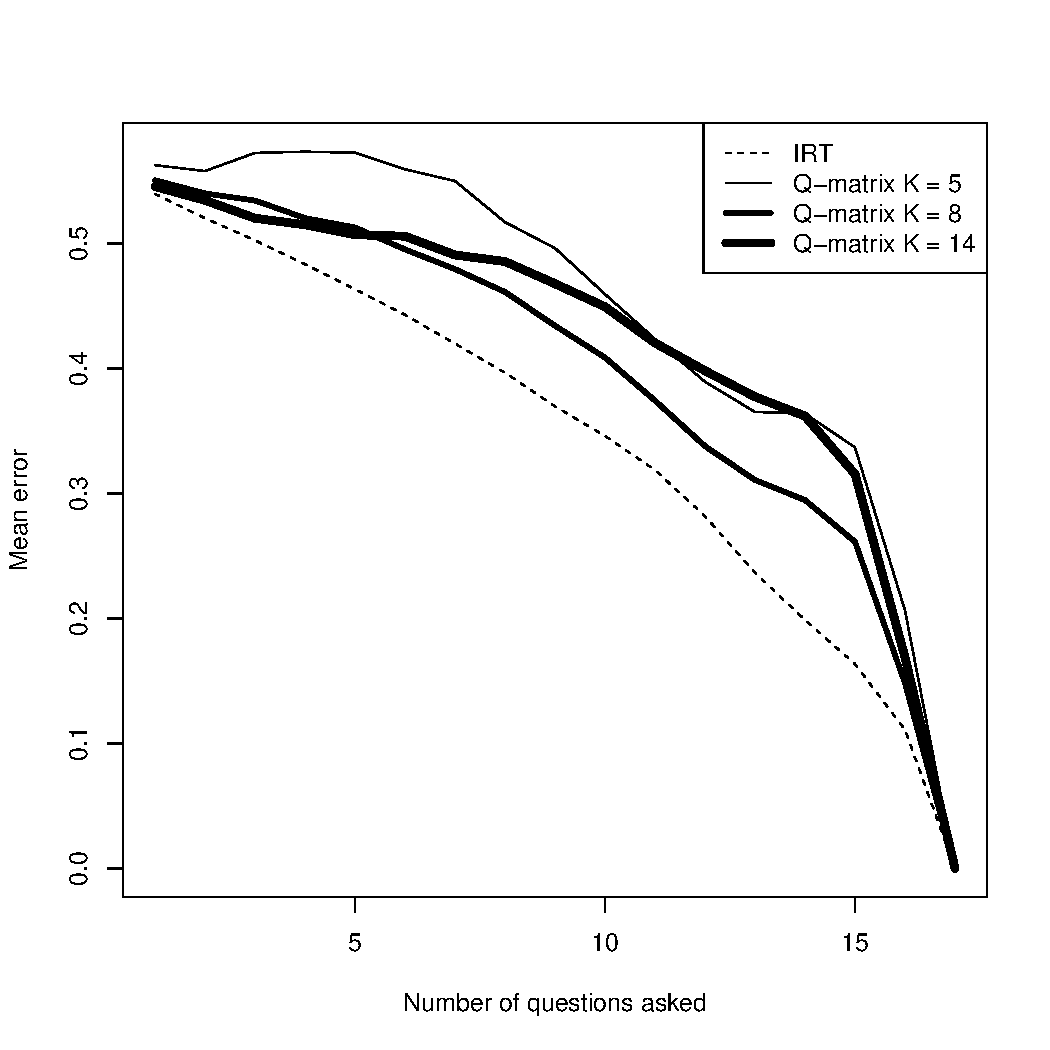
\includegraphics[width=0.49\linewidth]{castor.pdf}
\includegraphics[width=0.49\linewidth]{fraction.pdf}
%\includegraphics[width=0.33\linewidth]{sat.pdf}
\scriptsize\centering\begin{tabular}{@{}c|ccc@{}}
%& \multicolumn{3}{c}{Number of questions asked}\\
\textbf{Castor} & After 4 q. & After 10 q. & After 16 q.\\
\hline
\textsf{Q} $K = 2$ & 0.555 $\pm$ 0.004 & 0.456 $\pm$ 0.005 & 0.167 $\pm$ 0.012 \\
\textsf{Q} $K = 5$ & 0.574 $\pm$ 0.004 & 0.460 $\pm$ 0.006 & 0.206 $\pm$ 0.016 \\
\textsf{Q} $K = 8$ & 0.520 $\pm$ 0.004 & 0.409 $\pm$ 0.006 & 0.148 $\pm$ 0.013 \\
\textsf{Q} $K = 11$ & 0.519 $\pm$ 0.004 & 0.462 $\pm$ 0.007 & 0.218 $\pm$ 0.014 \\
\textsf{Q} $K = 14$ & 0.515 $\pm$ 0.003 & 0.449 $\pm$ 0.006 & 0.169 $\pm$ 0.014 \\
\textsf{IRT} & \textbf{0.484 $\pm$ \textbf0.003} & \textbf{0.346 $\pm$ 0.005} & \textbf{0.111 $\pm$ 0.010} \\
\end{tabular}

\begin{tabular}{@{}c|ccc@{}}
%& \multicolumn{3}{c}{Number of questions asked}\\
\textbf{Fraction}\\%& After 4 q. & After 10 q. & After 16 q.\\
\hline
\textsf{Q} $K = 2$ & 0.464 $\pm$ 0.012 & 0.326 $\pm$ 0.013 & 0.196 $\pm$ 0.017 \\
\textsf{Q} $K = 5$ & 0.440 $\pm$ 0.011 & 0.289 $\pm$ 0.014 & \textbf{0.146 $\pm$ 0.013} \\
\textsf{Q} $K = 8$ & 0.407 $\pm$ 0.011 & 0.276 $\pm$ 0.015 & 0.159 $\pm$ 0.015 \\
\textsf{Q} $K = 11$ & \textbf{0.395 $\pm$ 0.009} & \textbf{0.255 $\pm$ 0.013} & 0.156 $\pm$ 0.015 \\
\textsf{Q} $K = 14$ & 0.422 $\pm$ 0.009 & 0.274 $\pm$ 0.014 & 0.180 $\pm$ 0.018 \\
\textsf{IRT} & 0.435 $\pm$ 0.012 & 0.304 $\pm$ 0.013 & \textbf{0.142 $\pm$ 0.012} \\
\textsf{Q*} $K = 8$ & 0.596 $\pm$ 0.008 & 0.346 $\pm$ 0.007 & 0.182 $\pm$ 0.007 \\
\end{tabular}

\begin{tabular}{@{}c|ccc@{}}
%& \multicolumn{3}{c}{Number of questions asked}\\
\textbf{SAT}\\%& After 4 q. & After 10 q. & After 16 q.\\
\hline
\textsf{Q} $K = 2$ & 0.522 $\pm$ 0.007 & 0.417 $\pm$ 0.010 & 0.315 $\pm$ 0.018 \\
\textsf{Q} $K = 5$ & 0.469 $\pm$ 0.007 & 0.365 $\pm$ 0.012 & 0.306 $\pm$ 0.019 \\
\textsf{Q} $K = 8$ & 0.463 $\pm$ 0.007 & 0.367 $\pm$ 0.013 & \textbf{0.242 $\pm$ 0.018} \\
\textsf{Q} $K = 11$ & 0.456 $\pm$ 0.008 & 0.364 $\pm$ 0.013 & 0.331 $\pm$ 0.023 \\
\textsf{Q} $K = 14$ & 0.441 $\pm$ 0.007 & 0.350 $\pm$ 0.012 & 0.296 $\pm$ 0.021 \\
\textsf{IRT} & \textbf{0.409 $\pm$ 0.008} & \textbf{0.285 $\pm$ 0.012} & \textbf{0.248 $\pm$ 0.022} \\
\end{tabular}
\caption{Mean error of the different algorithms over the remaining questions of the Castor, Fraction and SAT datasets, after a certain number of questions have been asked. In the figure above, the dashed curve denotes the Rasch model (\textsf{IRT}), while the curves of growing thickness denote q-matrices (\textsf{Q}) of growing number of columns. The dotted curve in Fraction denotes the handmade q-matrix (\textsf{Q*})~\cite{DeCarlo2010}.}\vspace*{-5mm}
\label{tab:castor}
\end{table}

\section{Acknowledgements}

We thank Chia-Tche Chang, Le Thanh Dung Nguyen and especially Antoine Amarilli for their valuable comments. We also thank Mathias Hiron for providing the Castor dataset. This work is supported by the Paris-Saclay Institut de la Société Numérique funded by the IDEX Paris-Saclay, ANR-11-IDEX-0003-02.\vspace{-2.5mm}

%
% The following two commands are all you need in the
% initial runs of your .tex file to
% produce the bibliography for the citations in your paper.
\bibliographystyle{abbrv}
\small\bibliography{sigproc}  % sigproc.bib is the name of the Bibliography in this case
% You must have a proper ".bib" file
%  and remember to run:
% latex bibtex latex latex
% to resolve all references
%
% ACM needs 'a single self-contained file'!
%
%APPENDICES are optional
%\balancecolumns
% That's all folks!
\end{document}
